\section{Object 1}
\markright{Object 1}

\subsubsection{Part 1}

The primary structural component was modeled using basic sketching and extrusion features to establish the overall geometry. Dimensional constraints were applied to ensure precise dimensions, and fillets were added to reduce stress concentrations at sharp edges. This part serves as the foundational element upon which other components are mounted.

\begin{figure}[H]
	\centering
	\begin{subfigure}[b]{0.4\textwidth}
		\centering
		
\includegraphics[width=\textwidth, keepaspectratio]{lab-03/assets/1/1.jpg}
	\end{subfigure}%
	\hspace{0.3em}
	\begin{subfigure}[b]{0.4\textwidth}
		\centering
		
\includegraphics[width=\textwidth, keepaspectratio]{lab-03/assets/1/2.jpg}
	\end{subfigure}%
	\caption{Snapshots while Designing Part 1 of Object 1 in Solidworks}
	\label{lab03_object_1_part_1}
\end{figure}

\subsubsection{Part 2}

This component was designed with features that enable controlled motion and load transmission. Multiple circular profiles and stepped geometries were created using revolve and pocket features to achieve the required functionality. Tolerance specifications were incorporated to ensure proper fit and operation with mating components.

\begin{figure}[H]
	\centering
	\begin{subfigure}[b]{0.4\textwidth}
		\centering
		
\includegraphics[width=\textwidth, keepaspectratio]{lab-03/assets/1/3.jpg}
	\end{subfigure}%
	\hspace{0.3em}
	\begin{subfigure}[b]{0.4\textwidth}
		\centering
		
\includegraphics[width=\textwidth, keepaspectratio]{lab-03/assets/1/4.jpg}
	\end{subfigure}%
	\caption{Snapshots while Designing Part 2 of Object 1 in Solidworks}
	\label{lab03_object_1_part_2}
\end{figure}

\subsubsection{Part 3}

A cylindrical element with specific geometric features was modeled to facilitate rotational and translational motion within the assembly. Extrude and revolve features were used to create the core geometry, while bore holes were incorporated using pocket features. The part was designed with appropriate surfaces for bearing interfaces and load distribution.

\begin{figure}[H]
	\centering
	\begin{subfigure}[b]{0.4\textwidth}
		\centering
		
\includegraphics[width=\textwidth, keepaspectratio]{lab-03/assets/1/5.jpg}
	\end{subfigure}%
	\hspace{0.3em}
	\begin{subfigure}[b]{0.4\textwidth}
		\centering
		
\includegraphics[width=\textwidth, keepaspectratio]{lab-03/assets/1/6.jpg}
	\end{subfigure}%
	\caption{Snapshots while Designing Part 3 of Object 1 in Solidworks}
	\label{lab03_object_1_part_3}
\end{figure}

\subsubsection{Part 4}

This auxiliary component was created to provide structural support and alignment for the assembly mechanism. Sketch-based features and simple extrusions were used to establish its geometry, with dimensional constraints ensuring compatibility with the other parts. Surface finish specifications and mounting points were carefully defined.

\begin{figure}[H]
	\centering
	\begin{subfigure}[b]{0.35\textwidth}
		\centering
		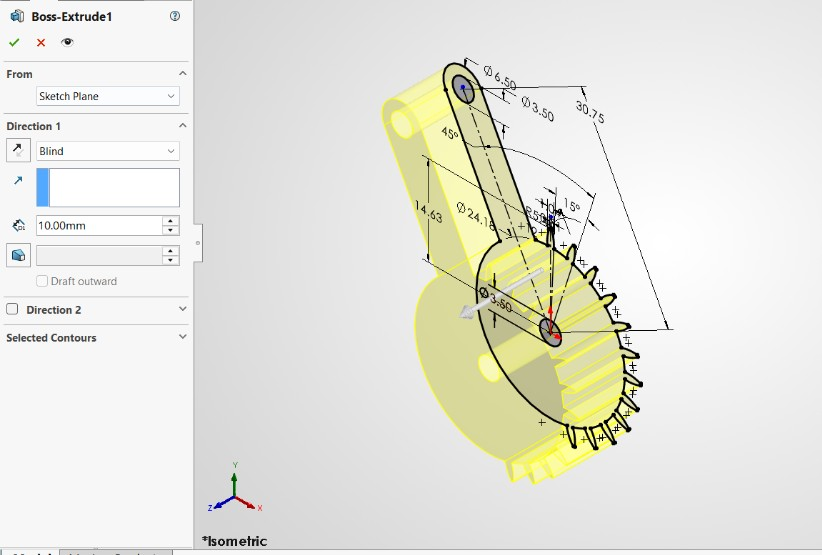
\includegraphics[width=\textwidth, keepaspectratio]{lab-03/assets/1/7.jpg}
	\end{subfigure}%
	\hspace{0.3em}
	\begin{subfigure}[b]{0.35\textwidth}
		\centering
		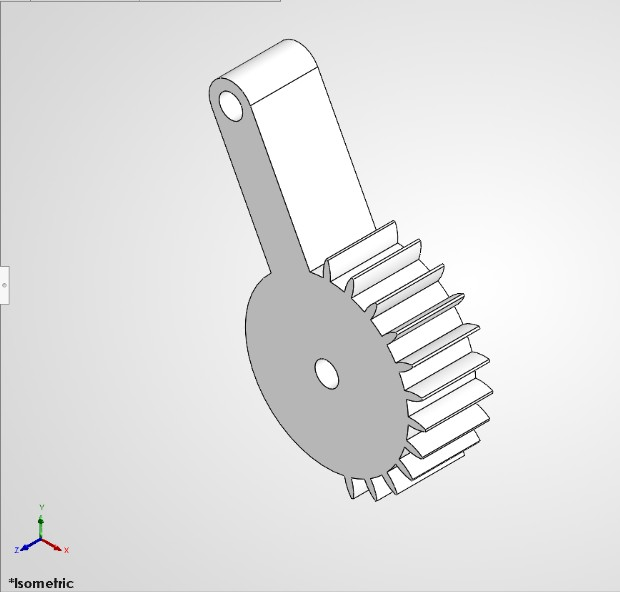
\includegraphics[width=\textwidth, keepaspectratio]{lab-03/assets/1/8.jpg}
	\end{subfigure}%
	\caption{Snapshots while Designing Part 4 of Object 1 in Solidworks}
	\label{lab03_object_1_part_4}
\end{figure}

\subsubsection{Assembly}

All four components were assembled using coincident and distance constraints to define the relative positions and allow for controlled motion between parts. Kinematic constraints were verified to ensure that the assembly mechanism functions as intended without interference or overlap. The final assembly was visualized from multiple angles to confirm proper alignment and motion characteristics.

\begin{figure}[H]
	\centering
	\begin{subfigure}[b]{0.35\textwidth}
		\centering
		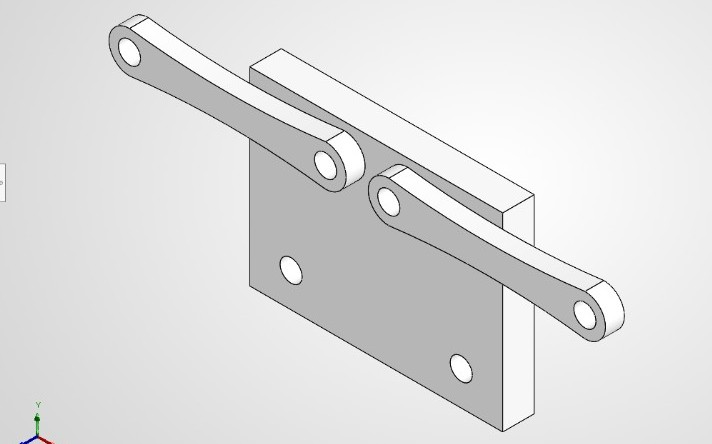
\includegraphics[width=\textwidth, keepaspectratio]{lab-03/assets/1/9.jpg}
	\end{subfigure}%
	\hspace{0.3em}
	\begin{subfigure}[b]{0.35\textwidth}
		\centering
		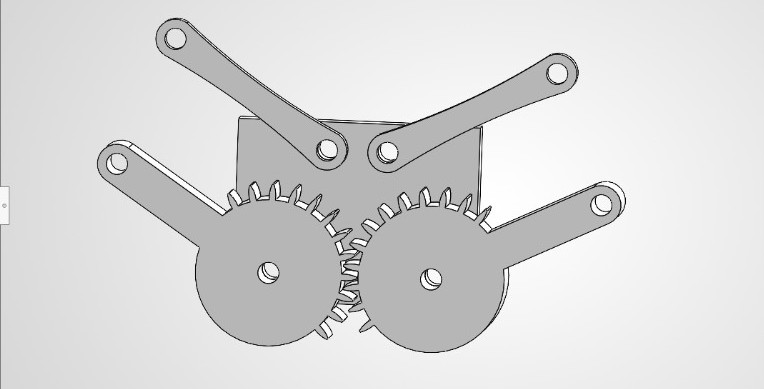
\includegraphics[width=\textwidth, keepaspectratio]{lab-03/assets/1/10.jpg}
	\end{subfigure}%
	\vspace{0.3em}
	\begin{subfigure}[b]{0.7\textwidth}
		\centering
		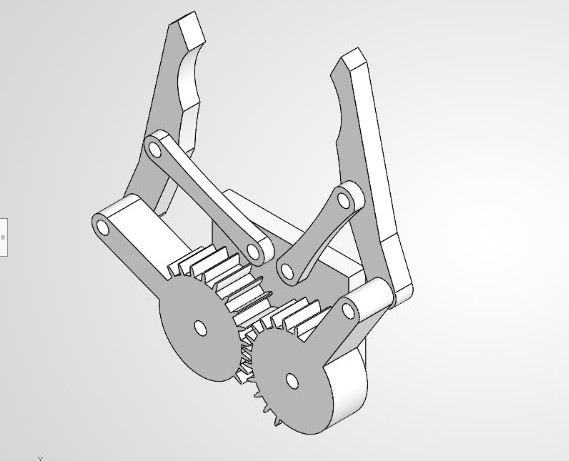
\includegraphics[width=\textwidth, keepaspectratio]{lab-03/assets/1/11.jpg}
	\end{subfigure}%
	\caption{Snapshots while Assembling Object 1 in Solidworks}
	\label{lab03_object_1_assembly}
\end{figure}

